\documentclass[]{article}
\usepackage[margin=1cm]{geometry}
\usepackage{tikz,pgfplots,pgf}
\usetikzlibrary{matrix,shapes,arrows,positioning}
\usepackage{Sweave}
\begin{document}
\Sconcordance{concordance:nn-04.tex:nn-04.Rnw:%
1 4 1 1 0 60 1}


\begin{figure}[htp]
\centering
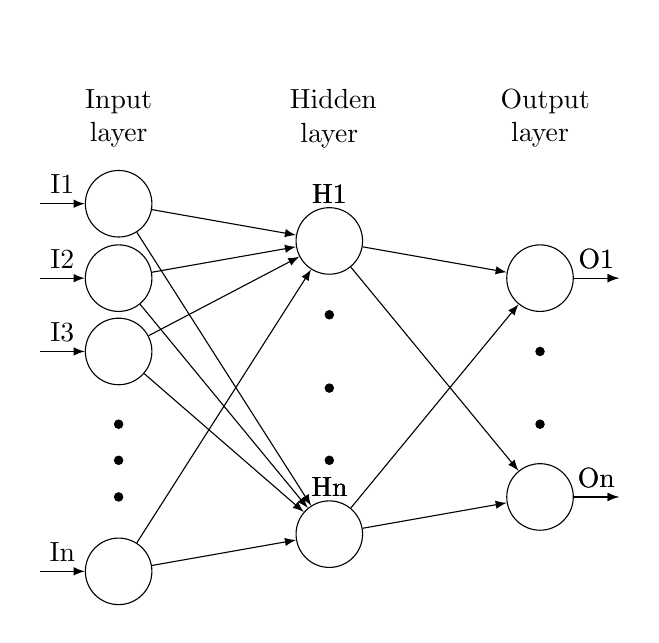
\begin{tikzpicture}[
plain/.style={
  draw=none,
  fill=none,
  },
dot/.style={draw,shape=circle,minimum size=3pt,inner sep=0,fill=black
  },
net/.style={
  matrix of nodes,
  nodes={
    draw,
    circle,
    inner sep=8.5pt
    },
  nodes in empty cells,
  column sep=0.6cm,
  row sep=-11pt
  },
>=latex
]
\matrix[net] (mat)
{
|[plain]| \parbox{1cm}{\centering Input\\layer} 
          & |[plain]| \parbox{1cm}{\centering Hidden\\layer} 
                       & |[plain]| \parbox{1cm}{\centering Output\\layer} \\
          & |[plain]|                 \\
|[plain]| &            & |[plain]|    \\
          & |[plain]|  &              \\
|[plain]| & |[dot]|                   \\
          & |[plain]|  & |[dot]|      \\
|[plain]| & |[dot]|    & |[plain]|    \\
|[dot]|   & |[plain]|  & |[dot]|      \\
|[dot]|   & |[dot]|    & |[plain]|    \\
|[dot]|   & |[plain]|  &              \\
|[plain]| &            & |[plain]|    \\
          & |[plain]|                 \\
};
\foreach \ai/\mi in {2/I1,4/I2,6/I3,12/In}
  \draw[<-] (mat-\ai-1) -- node[above] {\mi} +(-1cm,0);
\foreach \ai in {2,4,6,12}
{\foreach \aii/\mii in {3/H1,11/Hn}
  \draw[->] (mat-\ai-1) -- (mat-\aii-2) node[yshift=0.6cm] {\mii};
}
\foreach \ai in {3,11}
{  \draw[->] (mat-\ai-2) -- (mat-4-3);
  \draw[->] (mat-4-3) -- node[above] {O1} +(1cm,0);}
\foreach \ai in {3,11}
{  \draw[->] (mat-\ai-2) -- (mat-10-3);
  \draw[->] (mat-10-3) -- node[above] {On} +(1cm,0);}
\end{tikzpicture}

\caption{ANN diagram for Speed Sign recognition.}
\label{fig_m_3}
\end{figure}

\end{document}
